\section{Battery Safety}
\label{Chap:Battery_Safety}
\subsection{Thermal Runaway}
Batteries are high-density energy storing devices. Energy stored in batteries is ideally released at a limited rate to power a device via an electronic circuit. The release of too much energy however leads to potentially dangerous situations. In this section it is explained why lithium-ion batteries are so susceptible to damage. It then is explored what measures can be taken to extend safety and lifetime.

The problem of almost all energy cells is that these cells have the ability to rapidly generate heat from exothermic chemical reactions that fuel new exothermic reactions and cause a so called 'thermal runaway'. With lithium-ion batteries, the intensity of the thermal runaway is worse than most other battery chemistries. Lithium-ion batteries are more energy-dense and during a thermal runaway, the stored energy will fuel the runaway. Additionally, the electrolyte used in lithium batteries is a flammable liquid that ignites easily\cite{Mikolajczak2011}. Thermal runaway is started when the cell produces more heat than it loses, even when electrically cut-off. This can thus be from a high ambient temperature or a high internal current flow (like with internal shorting),  starting chemical decomposition in the cell.

\subsubsection{Battery Decomposition}
The chemical decomposition, and thus thermal runaway, starts at around 80-100\textit{$\degree C$}. A thin layer called the Solid-Electrolyte-Interface (SEI) is exothermically decomposed\cite{FENG2018246}. This layer forms during the initial charge of the battery cell by charged electrode-electrolyte contact. The layer protects the electrodes from reacting with the electrolyte like aluminum-oxide prevents aluminum from reacting with air. The electrodes are exposed to the electrolyte and its solvent after decomposition of the SEI. This forms no problem at temperatures below 200 \textit{$\degree C$}. Interestingly at this point, the SEI can even reform and stop the runaway, depending on the cells ability to dissipate heat\cite{FENG2018246}. \\  
At around 130\textit{$\degree C$} for Polyethylene (PE) separators or 170\textit{$\degree C$} for Polypropylene (PP) separators, the next event is triggered. The separator is decomposed, exposing the electrodes to one another initiating an internal short circuit\cite{Mikolajczak2011}\cite{FENG2018246}. Depending on the State-Of-Charge (SOC) of the cell and total capacity, the heat generated from this short circuit can be fierce, or could have an only mild effect. The short circuit renders the cell unusable since no potential difference can be induced, and thus no voltage. Reaching separator decomposition temperature (for most commercial cells this will be 130\textit{$\degree C$}), a serious risk of thermal runaway is presented. This temperature is to be absolutely avoided.

\subsubsection{Runaway}
If together with the SEI decomposition and the internal short circuit a temperature of around 200\textit{$\degree C$} is reached, the electrodes and electrolyte react and decompose exothermically to reach temperatures of 600\textit{$\degree C$}. The decomposition produces heat as well as gas. The gas production builds op pressure, until the battery seal or casing fails. The gas now vents through the failure at high temperatures. If an ignition source and enough oxygen is presented, a fire or explosion can happen. If not, a black smoke venting out the battery is observed. The ignition source can be hot metal from the current collectors or the hot cell casing (possibly created from local friction between the venting gas and the casing). This will ignite the decomposition gases and the remaining flammable electrolyte\cite{Mikolajczak2011}. In figure \ref{Fig:Thermal_Runaway} a thermal runaway of a pouch cell can be seen.

\begin{figure} [H]
	\centering
	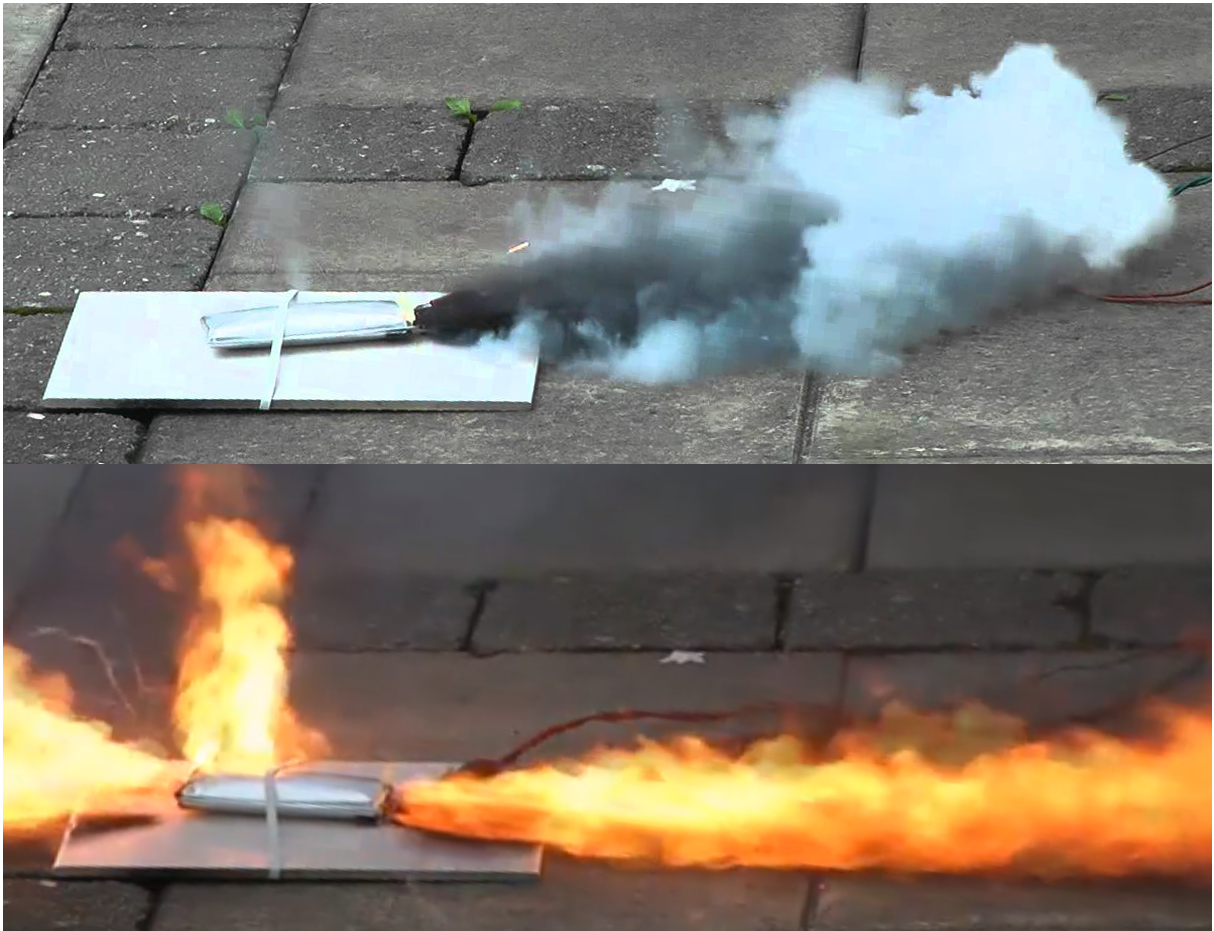
\includegraphics[width=0.4\linewidth]{Figures/pouch_failure.png}
	\caption{Thermal runaway of a pouch cell. Gas is initially vented and is eventually ignited.}
   \label{Fig:Thermal_Runaway}
\end{figure}

\subsection{Abuse}
\subsubsection{Mechanical Abuse}
Besides manufacturing errors, thermal runaway may happen from three types of abuse. Mechanical, electrical or thermal abuse. One may have effect or cause the next type of abuse to start, schematically illustrated in figure \ref{Fig:Abuse_Chain}. Mechanical abuse is when the cell is penetrated, critically bend, vibrated to point of failure or any other forceful event that caused the cell to structurally fail, causing a electrical short. The resistance to mechanical abuse depends on the type of container the battery is protected by. The electrically active material itself does not offer much of mechanical resistance. It is up to the designer of the application to adequately offer mechanical protection.
\begin{figure} [H]
	\centering
	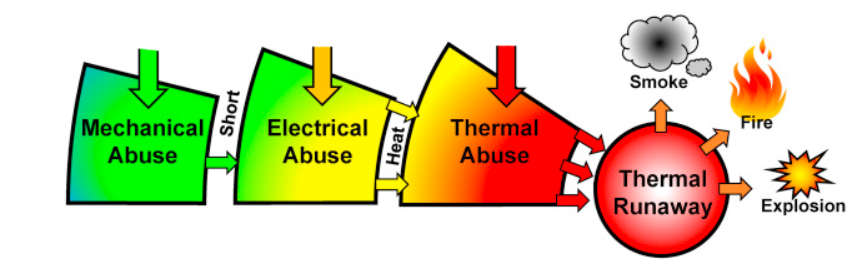
\includegraphics[width=0.6\linewidth]{Figures/abuse.png}
	\caption{Chain of abuse of a battery cell.}
   \label{Fig:Abuse_Chain}
\end{figure}
\subsubsection{Electrical Abuse}
\label{Sub:Electrical_Stability}
As described above, an internal short is fatal to a battery cell. However mechanical abuse is not the only trigger for an internal short. The cell can be charged or discharged too quickly, it can be charged with too much energy, or discharged too deeply. These might happen purposely because of demanding too much performance, or might happen accidentally by cell aging or imbalance.

\textit{Voltage Operating Window}\\
Charging or discharging a battery causes a change of voltage in the battery. A charged battery has a higher voltage than a discharged battery. All chemistries have their specific operating window, for most lithium chemistries this window is 4.2 - 2.5\textit{V}. However most battery suppliers provide this window on the battery's data-sheet and operate a smaller window of around 4.2 - 3\textit{V} for safety. Interestingly only the lower end of the window is often changed. This is because many chargers charge the cell via a constant current - constant voltage method, also called float charging, as illustrated in figure \ref{Fig:Charging} where the charging current decreases as the maximum voltage has been reached and floats at that voltage.
\begin{figure} [H]
	\centering
	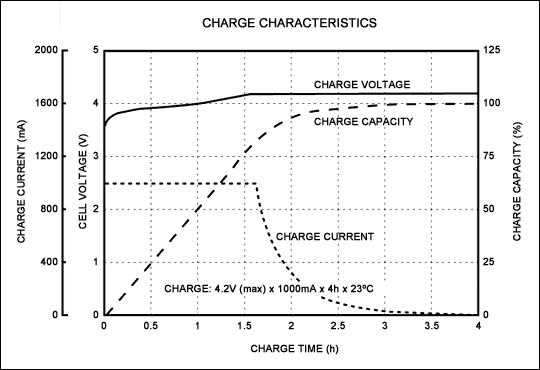
\includegraphics[width=0.8\linewidth]{Figures/charging.png}
	\caption{Constant current - constant voltage charging method.}
   \label{Fig:Charging}
\end{figure}
The lower limit however is importantly set to at least 3\textit{V}. To identify why this is, a discharge curve must be analyzed. A typical lithium battery discharge can be seen in figure \ref{Fig:Discharge}. A steep decline in voltage can be seen as the battery is nearing the discharge of all its capacity. Discharging more energy will quickly result to a sub 2.5\textit{V} voltage, damaging the battery and thus this margin is set. For the Solar Jet a warning should be given whenever this 3\textit{V} is reached to ensure enough capacity for landing.
\begin{figure} [H]
	\centering
	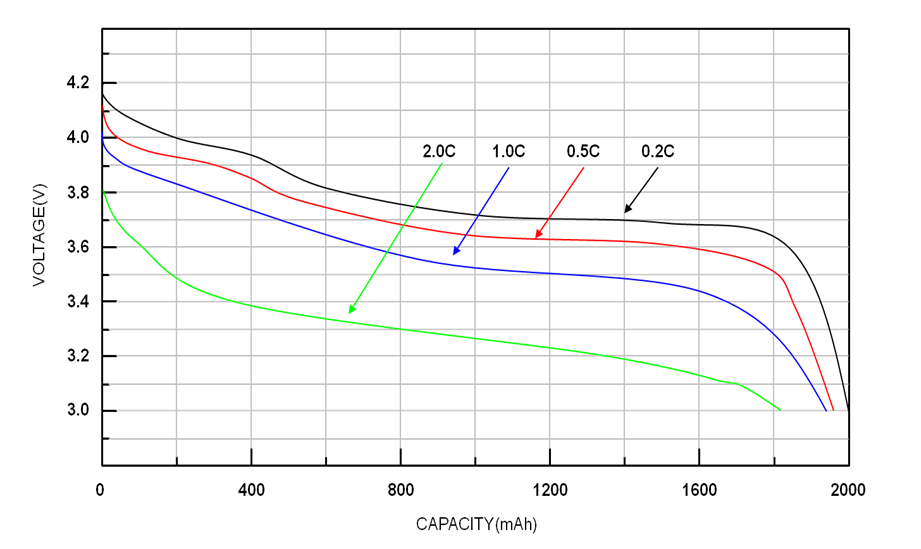
\includegraphics[width=0.65\linewidth]{Figures/battery-discharge.png}
	\caption{Typical lithium battery discharge curve.}
   \label{Fig:Discharge}
\end{figure}
Over(dis)charging damages the battery resulting in capacity and power loss. Worse is the increasing chance of internal short circuit and gas build up. Over(dis)charging deposits solid lithium normally dissolved in the electrolyte solvent on the electrodes. This can now react with the solvent producing gas. Additionally the deposition of solid metallics can cause dendrites (seen in figure \ref{Fig:Dendrite} to form that penetrate the separator, resulting in internal short circuit\cite{BIRKL2017373}. 
\begin{figure} [H]
	\centering
	
\includegraphics[width=0.5\linewidth]{Figures/Dendrites.jpg}
	\caption{Dendrite formation.}
   \label{Fig:Dendrite}
\end{figure}

\textit{Current Operating Window}\\
The operating window for the amount of current passing through the battery is decided by the battery's manufacturer. A manufacturer has to test the cell and follow safety regulations. After tests, finally a safe maximal continuous current draw will be set. Problematic is the fact that many battery suppliers provide a too high limit to increase theoretic performance.\\
A high current density results in more lithium deposition on the surface of active electrode material and thus prevents active material from intercalating than low current densities\cite{Arora19993543}. In figure \ref{Fig:Lithium_deposition} this effect can be seen. The result thus is worsening battery performance over time and dendrite formation. High currents also create more heat and thus during discharge less capacity is outputted since the additional heat loss. For safety, the Solar Jet team should always stay within the maximal continuous current window specified on the battery's data-sheet and preferably even maintain a safety factor. 
\begin{figure} [H]
	\centering
	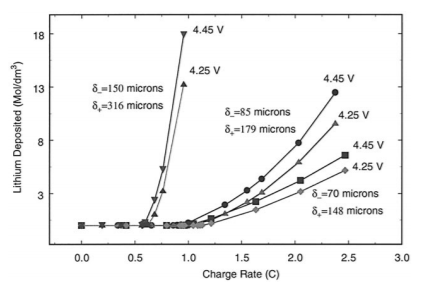
\includegraphics[width=0.7\linewidth]{Figures/charge_rate.PNG}
	\caption{Lithium deposition at different charge rates for different electrode thicknesses\cite{Arora19993543}.}
   \label{Fig:Lithium_deposition}
\end{figure}

\subsubsection{Thermal Abuse}
Thermal abuse is caused mostly by internal short circuit. However, a battery that discharges quickly, can heat up by internal resistance as well if it drains for an extended period of time. An analysis of the heat generation of discharging the battery selected in \ref{Chap:Battery_Selection} is conducted in \ref{Chap:thermal_model}. Thermal abuse can be internal, just as well as external. When the battery is either used or stored in a too high or low ambient temperature, the battery can be damaged. A too high temperature, again starts chemical decomposition. A too low temperature can be critical as well. Because the intercalation process at low temperatures (below 0\textit{$\degree C$}) does not perform very well, lithium deposits on the anode. This again causes performance loss and possible internal short circuit\cite{Petzl2015}. Especially during the charging process the temperature should be above freezing temperature.

\subsection{Safety Measures}
\label{Safety_measures}
\subsubsection{Voltage and current control}
Probably the most important safety measure besides mechanical stability is a way of measuring the voltage over the battery pack in the Solar Jet. Dropping below the specified voltage can be fatal. To measure the voltage over the battery pack, the voltage can be measured off each individual cell, or all cells combined. Preferably all cells are monitored individually as all cells will slightly differ from each other, which can lead to one cell degrading quickly compared to the others. A total pack voltage can than be generated by summing all battery voltages to indicate pack state of charge. 

Monitoring all cell the cells can be done with a Battery Monitoring System (BMS). The BMS is fed small cables from all series connections as seen in figure \ref{Fig:Wiring_Scheme}. Now the BMS is connected in parallel to the electronic circuit and acts as a regular volt meter by looking at the potential difference over a high resistance. 
\begin{figure} [H]
	\centering
	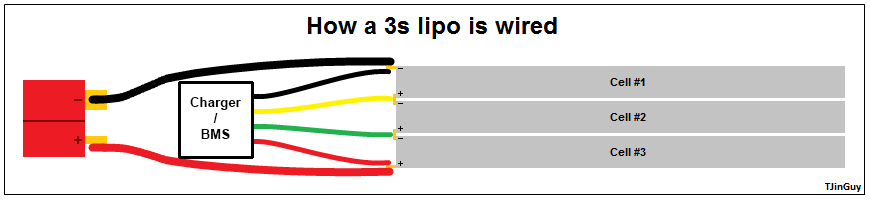
\includegraphics[width=0.8\linewidth]{Figures/balancing.png}
	\caption{Wiring scheme for setting up a BMS or a balancing charger}
   \label{Fig:Wiring_Scheme}
\end{figure}
A problem however is that no monitoring circuitry was found that can handle 14s 180\textit{A}. Only Protection Circuit Boards (PCB's) were found. These protection devices can not be read, these only shut down the circuit if needed. A device that can be read however is the Mauch HS-200-HV Voltage and Current Sense Board\cite{Mauch}. This device can only be reading out the total voltage, so the individual cell measurement functionality is lost. The upside is that the Mauch chip works with the Pixhawk flight computer currently used in the Solar Jet project. The Mauch chip measures the current with a hall sensor able to handle 200\textit{A}. The voltage is measured by using a voltage divider of 1:18. This is because the Pixhawk may only receive 3.3\textit{V} as maximal voltage input for voltage measurement. The maximal amount of lithium batteries can now be calculated. The maximal allowable voltage over the chip is:
\begin{equation}
V_{max} = V_{Pixhawk} \cdot \frac{R_l}{R_s} = 3.3 \cdot \frac{18}{1} = 59.4\textit{V} 
\end{equation}
With $R_s$ being the small resistance and $R_l$ the large resistance in the resistance divider.\\
Now the number of cells can be calculated by using the maximal voltage that should be put into a cell.
\begin{equation}
\frac{V_{max}}{V_{cell}} = \frac{59.4}{4.2} = 14
\end{equation}
The Mauch chip needs to be powered, but in turn can power the Pixhawk as well. The Mauch chip needs 5.35\textit{V} and 3\textit{A} just like the Pixhawk. Via a Battery Elimination Circuit (BEC) also from Mauch, power can be drawn from dedicated batteries for the Pixhawk, or from the main batteries powering the motor. This BEC reduces the voltage and current to the necessary 5.35\textit{V} and 3\textit{A}. The BEC connects to the Mauch Chip. The Mauch chip then connects to the pixhawk with 5 wires: the ground, two power cables and a volt and current measurement cable. A wiring scheme can be seen in figure \ref{Fig:BMS}.
\begin{figure} [H]
	\centering
	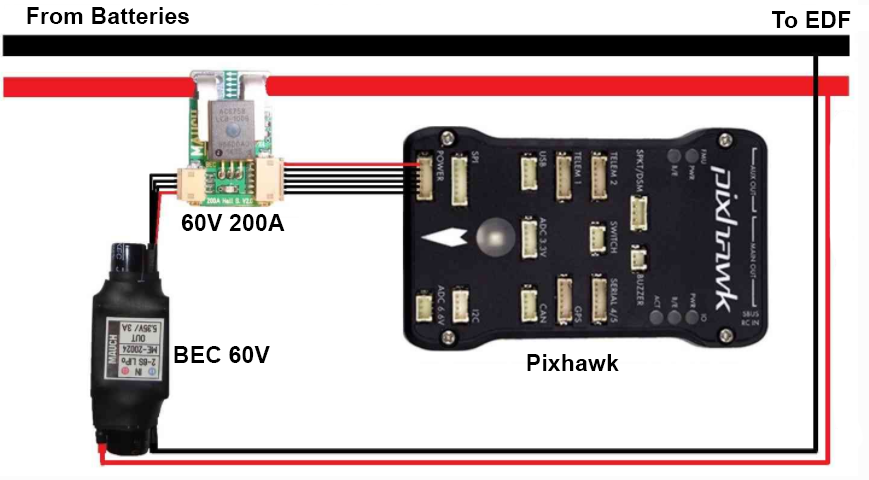
\includegraphics[width=0.5\linewidth]{Figures/BMS.PNG}
	\caption{Setup of Mauch HS-200-HV, BEC-HV and Pixhawk monitoring system.}
   \label{Fig:BMS}
\end{figure}
With the data delivered to the Pixhawk, software can now be written to either reduce the power to the EDF as to indicate the battery is almost empty or to indicate a battery problem for example.

The Mauch BEC-HV\cite{Mauch2} and the Mauch HS-200-HV\cite{Mauch1} cost \euro45,- in total.


\subsubsection{Charging}
Charging should always be done at the specified current as indicated in the battery's data-sheet, or even slower. Lithium batteries are especially vulnerable to lithium deposit during charge thus this should never be rushed or conducted in hostile temperatures, for reasons mentioned earlier.

Another factor to keep in mind is the fact cells may be imbalanced after discharge or storage. This is important since imbalanced cells will degrade more quickly. A cell with less capacity, charges to 4.2\textit{V} faster, and discharges to 2.5\textit{V} earlier than a cell with more capacity. This increases the chance of the cell being damaged, destroying its capacity even more. The current charger used, the Multiplex power peak d7 400w, is able to check all individual cells and can be used to balance them if needed. The wires of figure \ref{Fig:Wiring_Scheme} are used to connect the balance function of the charger to each individual battery cell.

\subsubsection{Storage}
Batteries slowly lose capacity over time. This is due to internal chemical reactions. The structured electrodes slowly decompose, change shape or react with the electrolyte or its solvent. Typically these reactions happen more quickly at an elevated temperature\cite{Keil2016}. Storing temperatures should thus be kept low, but should not be below zero\textit{$\degree C$}. Performance of lithium batteries significantly decrease below zero. Less capacity is charged and this may not recover well after warming up again\cite{Aris2017}. To keep a safe margin and meanwhile slow the self discharge process, it is advised to store the batteries around 15\textit{$\degree C$}. 

Not only temperature influences the self discharge process. State of charge is a major influence as well. Typically it is advised to store lithium batteries around 3.7\textit{V}. This is because for most batteries, a 50\% state of charge is reached when the cell is at around 3.8\textit{V} during a low speed discharge. This can also be observed for the discharge curve \ref{Fig:Discharge} given earlier. The 50\% charge is chosen since at around 60\% charge, for most battery chemistries a worsening in performance is examined. In figure \ref{Fig:SOC} this is clearly seen. It can also be noted that even less state of charge is even better, however this gives more chance for the battery to drop below 2.5\textit{V} accidentally. Also it can be seen that indeed a higher temperature decreases performance after ten months of storage.

\begin{figure} [H]
	\centering
	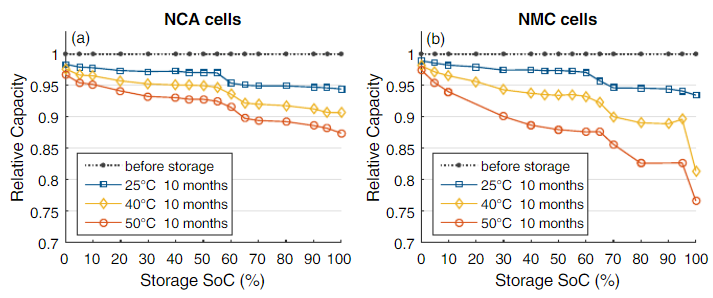
\includegraphics[width=0.8\linewidth]{Figures/SOC.PNG}
	\caption{Li-ion batteries stored for 10 months at different temperatures\cite{Keil2016}.}
   \label{Fig:SOC}
\end{figure}

%\begin{figure} [H]
% 	\centering
% 	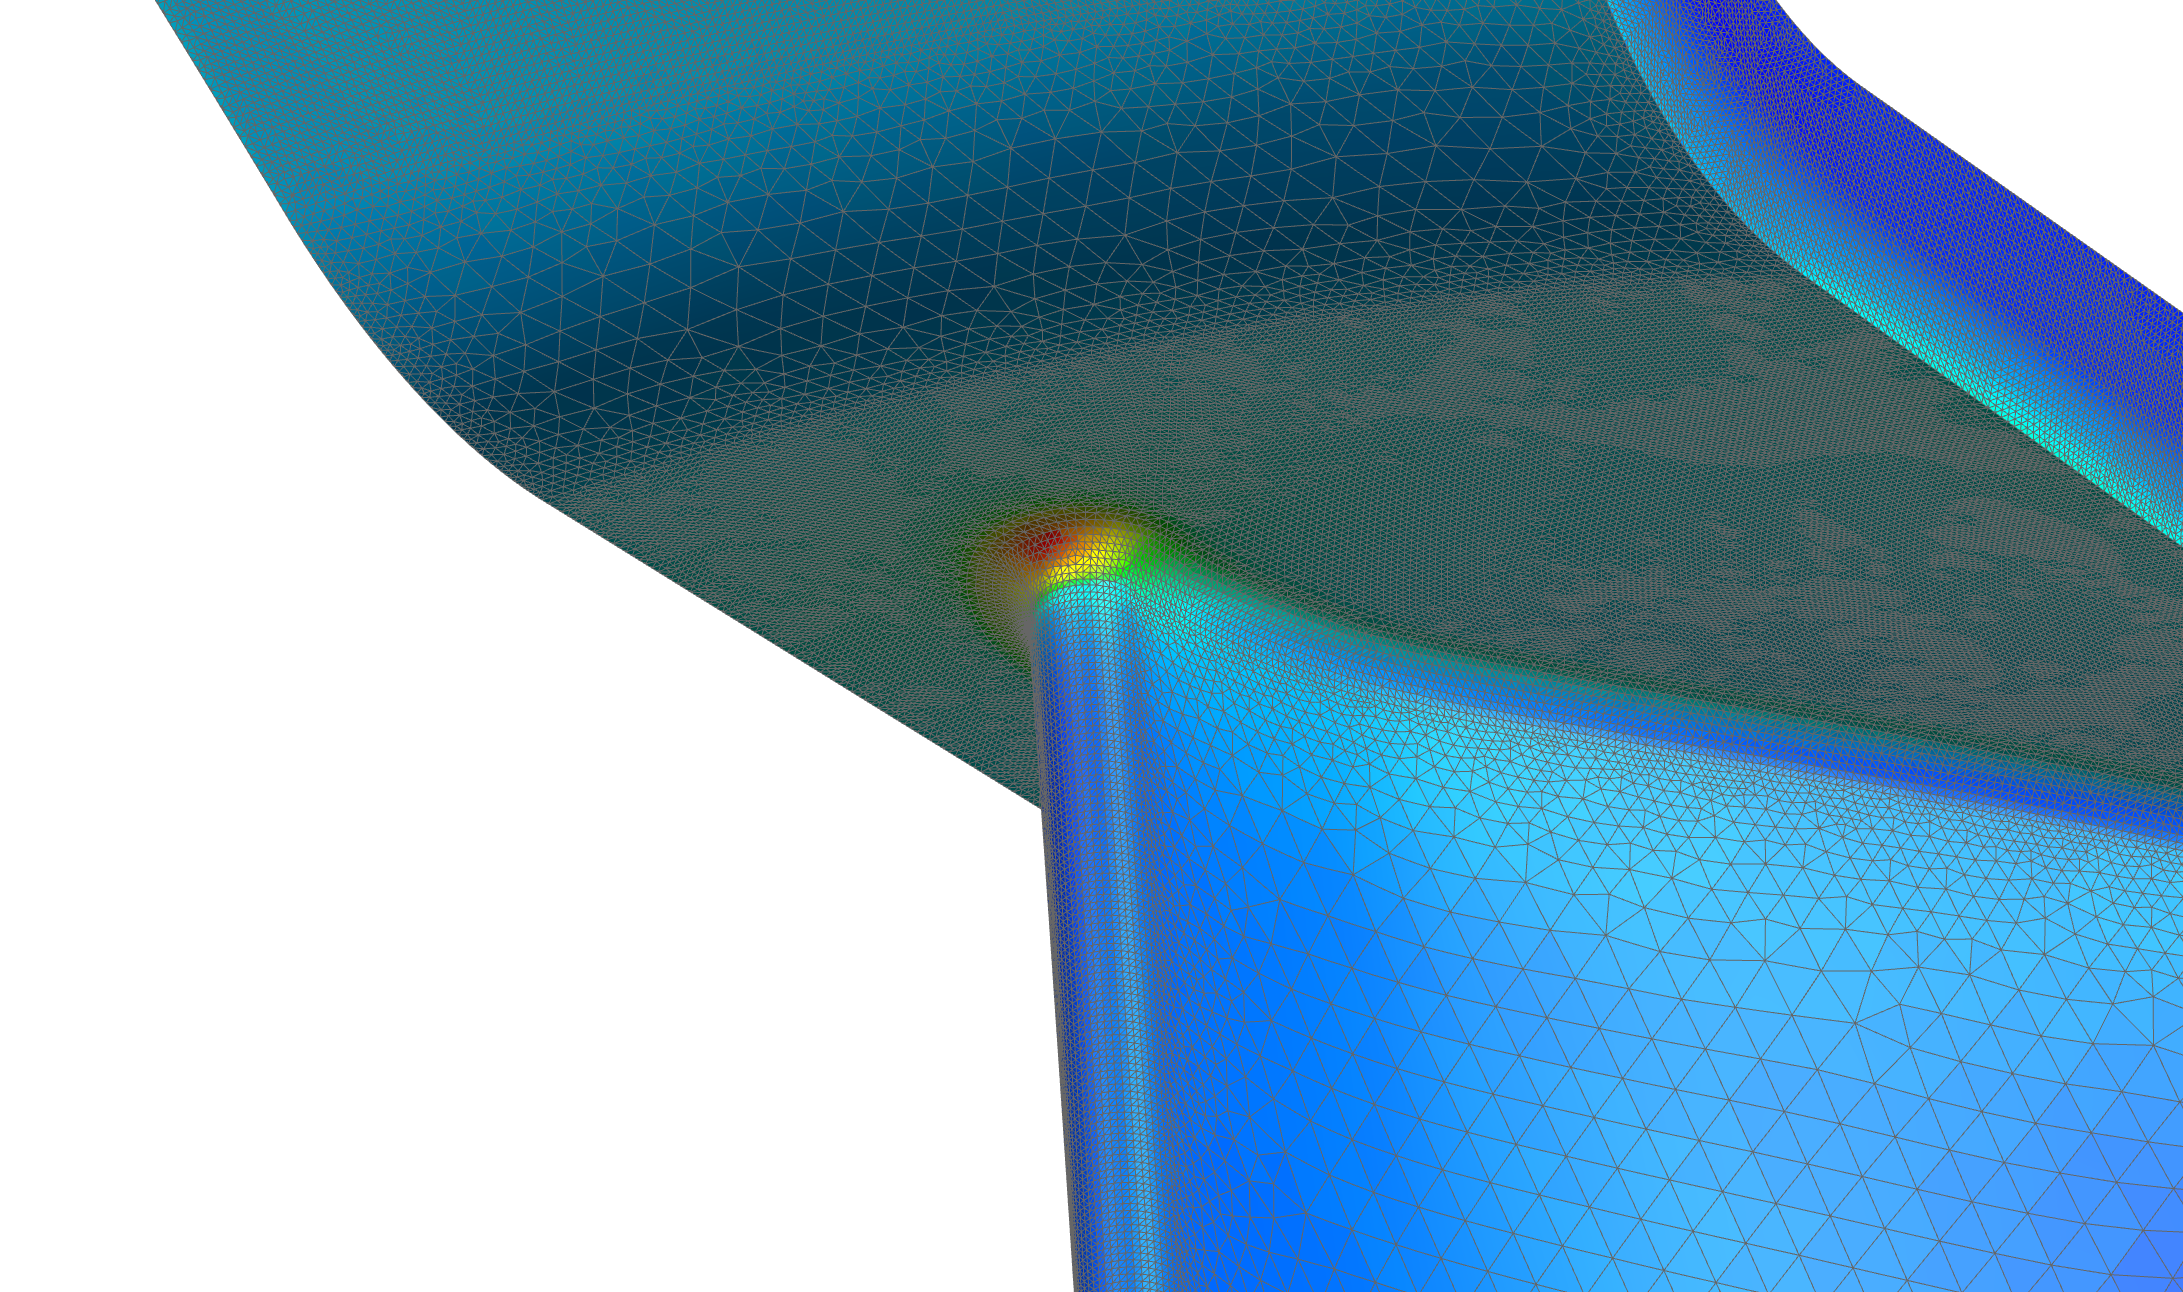
\includegraphics[width=0.8\linewidth]{Figures/stator_shutdown.png}
% 	\caption{Maximum stress during shut-down condition}
%    \label{stator1}
% \end{figure}

\newpage